%%% for platex
\documentclass[a4paper,12pt]{jbook}
%%% for lualatex
%\documentclass[a4paper,12pt]{ltjbook}

\usepackage{bachelor}
\usepackage{ipsj}
\usepackage{color}
\usepackage{amssymb}
\usepackage{amsmath}
\usepackage{amsthm}
\usepackage{multirow,bigdelim}
\newcommand{\la}{\leftarrow}
\newcommand{\Lra}{\Longrightarrow}
\newcommand{\Lla}{\Longleftarrow}
\newcommand{\Llra}{\Longleftrightarrow}
\newcommand{\lra}{\longrightarrow}
\newcommand{\dd}{\mathop{..}}
\newcommand{\range}[2]{\{#1\dd#2\}}
\newcommand{\imp}{\Rightarrow}
\newcommand{\equ}{\Leftrightarrow}
\renewcommand{\labelenumi}{(\arabic{enumi})}
\newcommand{\alldiff}{\textrm{alldifferent}}
\newcommand{\Alldiff}{\alldiff(x_1,x_2,\ldots,x_n)}
\newcommand{\SAT}{{\tt SAT}}
\newcommand{\UNSAT}{{\tt UNSAT}}
\newcommand{\Dom}{{\it Dom}}
% \newcommand{\p}[2]{p(#1,#2)}
\newcommand{\dE}[2]{p(#1=#2)}
\newcommand{\lE}[2]{p(#1^{(#2)})}
\newcommand{\oE}[2]{p(#1\le#2)}
 % 自分用のマクロ

%%%%%%%%%%%%%%%%%%%%%%%%%%%%%%%%%%%%%%%%%%%%%%%%%%%%%%%%%%
% タイトル
%%%%%%%%%%%%%%%%%%%%%%%%%%%%%%%%%%%%%%%%%%%%%%%%%%%%%%%%%%
\school{名古屋大学情報学部\\コンピュータ科学科}
\bookname{卒業論文}
\title{SMTソルバーにおける$distinct$制約の高速化とクイーングラフ彩色問題への応用}
\date{2020年2月}
\author{小菅 脩司}

%%%%%%%%%%%%%%%%%%%%%%%%%%%%%%%%%%%%%%%%%%%%%%%%%%%%%%%%%% 
% 本体
%%%%%%%%%%%%%%%%%%%%%%%%%%%%%%%%%%%%%%%%%%%%%%%%%%%%%%%%%% 
\begin{document}
\maketitle

%%%%%%%%%%%%%%%%%%%%%%%%%%%%%%%%%%%%%%%%%%%%%%%%%%%%%%%%%% 
\chapter*{概要}
\pagenumbering{roman}
%%%%%%%%%%%%%%%%%%%%%%%%%%%%%%%%%%%%%%%%%%%%%%%%%%%%%%%%%% 

% 表紙を情報工学コース用のスタイルにするために,作成した{\tt jbachelor.sty}が
% 必要である.
% TexStudioなどの便利なTex統合環境を利用するために,lualtexを使うとよい.
% platex と lualatex を切り替えるためには,このファイルの先頭を編集してlualatex用
% のltjbook.clsを使うようにする.
% \begin{verbatim}
% %%% for platex
% \documentclass[a4paper,12pt]{jbook}
% %%% for lualatex
% %\documentclass[a4paper,12pt]{ltjbook}
% \end{verbatim}

% 命題論理の充足可能性判定問題(Boolean SATisfiability; SAT)は,与えられ
% た命題論理式の充足可能性を判定する問題である.
% 近年,SAT の解を求める SAT ソルバーの性能が大きく向上し,
% SAT を拡張・発展させた問題を中心に,SAT 技術が大きな広がりを見せている.
%
% なかでも,
背景理論付き SAT (Satisfiability Modulo Theories; SMT) は,
背景理論が扱えるよ
うに,SAT を拡張・発展させた技術である.
SMT は,背景理論をより表現能力の高い述語論理で記述できるため,
問題を簡潔に記述することができる点が特長である.
% 近年,SAT ソルバー
% を拡張した高速 SMT ソルバーが開発され,制約充足問題,プログラム検証な
% どへの応用が活発に研究されている.

制約プログラミングの言語である制約充足問題は,与えられた制約を満たす解
を探索する問題である.
制約充足問題では,グローバル制約を用いて,複数の変数に対する複雑な
制約を簡潔に表現できる点が特長の一つである.
代表的なグローバル制約$distinct(x_{1},x_{2},\ldots x_{n})$は,
$x_{i}$が互いに異なる値をとることを表す.
この$distinct$制約は,記述性の向上を目的として SMT ソルバー
にも取り入れられている.
しかしながら,制約充足問題に対する SMT ソルバーの求解性能は,
SAT 型制約ソルバーと比べて劣っているとの報告もあり,
$distinct$制約を含めその効率的な実装は重要な研究課題となっている.

本論文では,クイーングラフ彩
色問題を題材とし,その SMT 符号化と$distinct$制約の高速化について述べる.
クイーングラフ彩色問題の SMT 符号化として,
色変数モデル,位置変数モデル,0-1変数モデル,ハイブリッドモデルを実装した.
また,$distinct$制約の高速化として,
色変数モデルと位置変数モデルでは,
SAT型制約ソルバーで有効性が示されている鳩の巣原理等に基づくヒント制約を追加した.
0-1変数モデルとハイブリッドモデルでは,
$distinct$制約のPB符号化[大野,2019]を応用し,探索空間の枝刈りを実装した.

クイーングラフ彩色問題($5\leq N \leq 13$)を用いた実行実験の結果,
色変数モデル+ヒント制約と位置変数モデル+ヒント制約が,$N=11$まで解を求め,最も良い性能を示した.
これにより,$distinct$制約の高速化について,
SATでのヒント制約が SMT においても有効であることが確認できた.
その一方で,チャネリング制約を用いたハイブリッドモデルは,
SMTソルバーの場合,求解性能が低下することが確認された.

%%% Local Variables:
%%% mode: japanese-latex
%%% TeX-master: "paper"
%%% End:
    % 概要

\tableofcontents    % 目次
\listoffigures      % 図の目次
\listoftables       % 表の目次
\lstlistoflistings  % コードの目次

% ここから「本文」
%%%%%%%%%%%%%%%%%%%%%%%%%%%%%%%%%%%%%%%%%%%%%%%%%%%%%%%%%% 
\chapter{緒論}

\pagenumbering{arabic}

\textbf{時間割問題} (Timetabling Problem) は,
求解困難な組合せ最適化問題の一種である.
この問題には,ハード制約とソフト制約が存在し,ソフト制約に違反するとペ
ナルティが与えられる.必ず満たすべきハード制約を満たしながら,ペナルティ
の総和を最小にするような解を求めることが目的である.
現状では,質の高い時間割を編成するために多くの人間の労力が費やされている.
このような背景から,時間割に関する国際会議
(Practice and Theory of Automated Timetabling; PATAT)
や国際時間割競技会 (International Timetabling Competition; ITC)
が開催され,時間割ソルバーの性能向上に貢献している.

\textbf{解集合プログラミング} (Answer Set Programming; ASP) 
\cite{%
  Baral03:cambridge,%
  Gelfond88:iclp,%
  Inoue08:jssst,%
  Niemela99:amai}
  は,
論理プログラミングから派生した宣言的プログラミングパラダイムの一つである.
ASP 言語は一階論理に基づく知識表現言語の一種であり,論理プログラムは
ASP のルールの有限集合である.ASP システムは論理プログラムから安定モデ
ル意味論に基づく解集合を計算するシステムである.
近年,SAT 技術を応用した高速 ASP システムが実現され,ロボット工学,シ
ステム生物学,システム検証,プランニングなど様々な分野への実用的応用が
急速に拡大している.

近年,\textbf{カリキュラムベース・コース時間割}
(Curriculum-based Course Timetabling; CB-CTT)
問題に対する ASP を用いた解法が提案され,成功を収めている
\cite{%
 banbara17:ramp}.
CB-CTT 問題は,大学等の1週間の講義スケジュールを求める問題であり,
最も研究が盛んな教育時間割問題の一つである.
ASP は系統的探索であることを活かして,未解決問題の最適値を決定するなど
優れた性能を示している.
しかし,その一方で,ソフト制約が多く含まれるような問題集において,
局所的探索を用いた解法より性能が劣っている場合が見られる.

この問題を解決するために,系統的探索と局所的探索を組み合わせた
\textbf{Large Neighborhood Prioritized Search} (LNPS)
\cite{%
 hayama19:kobe}
が提案されている.
LNPS は,暫定解に含まれる変数の値割り当ての一部をランダムに選んで取り
消し,他の値割り当てをなるべく維持したままで解を再構築する反復法の一種
である.
ASP を用いた LNPS の利点は,解の再構築を系統的探索で行え,値割り当てを
なるべく維持したままでの再構築が自然に実現できることである.
LNPS の性能は,
暫定解の一部をランダムに選んで取り消す destroy 演算子に依存するが,
十分な研究がなされてない.

本論文では,LNPS を用いたカリキュラムベース・コース時間割 (CB-CTT)
問題の解法について述べる.
CB-CTT に対する既存研究
\cite{%
 kiefer16:patat}
 を応用して,
3種類の destroy 演算子 (random, day-period, day-room) を実装した.
random が問題の性質をまったく利用しないのに対し,
day-period と day-room は CB-CTT のソフト制約を考慮して
暫定解の一部をランダムに選んで取り消す点が特長である.
%
提案手法の有効性を評価するために,国際時間割競技会 ITC-2007 のベンチマー
ク問題(21問)を用いて実行実験を行った.その結果,
多くの問題に対して,day-period と day-room が既存 ASP 解法より良い解を
生成し,提案手法の有効性が確認できた.

以降の構成は以下の通りである.
第二章で時間割問題,特に本論文が対象とするカリキュラムベース・コース時
間割問題について述べる.
第三章で解集合プログラミングについて述べ,その中で,LNPS の実装におい
て重要な変数選択ヒューリスティクスの変更機能について述べる.
第四章で LNPS 及び 実装した destroy 演算について述べる.
第五章でカリキュラムベース・コース時間割問題に実装解法を適用した実験の
結果を述べ,既存 ASP との比較や,destroy 演算同士での比較を交え考察を
行う.
最後に第六章で結論を述べる.

%%%%%%%%%%%%%%%%%%%%%%%%%%%%%%%%%%%%%%%%%%%%%%%%%%%%%%%%%% 


%%% Local Variables:
%%% mode: latex
%%% TeX-master: "paper"
%%% End:

\chapter{SMTとSMTソルバー}\label{chap:smt}

\section{SMTとは}
\section{SMTソルバーとは}
\section{プログラム例}

%%% Local Variables:
%%% mode: japanese-latex
%%% TeX-master: "paper"
%%% End:

%%%%%%%%%%%%%%%%%%%%%%%%%%%%%%%%%%%%%%%%%%%%%%%%%%%%%%%%%% 
\chapter{グラフ彩色問題とその関連問題}
%%%%%%%%%%%%%%%%%%%%%%%%%%%%%%%%%%%%%%%%%%%%%%%%%%%%%%%%%%

%%%%%%%%%%%%%%%%%%%%%%%%%%%%%%%%%
\begin{figure}[tb]
  \begin{tabular}{cc}
    \begin{minipage}[t]{0.5\linewidth}
      \centering
      \includegraphics[keepaspectratio,clip,scale=0.2]{fig/order3.png}
      \caption{~\code{order}3の~\code{McGregor}~グラフ}
      \label{fig:order3}
    \end{minipage}
    \begin{minipage}[t]{0.5\linewidth}
      \centering
      \includegraphics[keepaspectratio,clip,scale=0.2]{fig/order3_mult.png}
      \caption{多色頂点数最大化問題の解の割当て}
      \label{fig:order3mult}
    \end{minipage}
  \end{tabular}
\end{figure}
%%%%%%%%%%%%%%%%%%%%%%%%%%%%%%%%%

グラフの各頂点を隣接する頂点と異なる色で彩色することを
\textbf{グラフ彩色問題(Graph Coloring)}と呼ぶ.
以下に本論文で対象となる問題群について述べる.

\begin{itemize}
\item \textbf{グラフ彩色判定問題}は
  与えられたグラフと色数に対してグラフ点彩色が可能かどうかを判定する問題である.
\item \textbf{グラフ彩色における同色頂点数最小化問題}は
  グラフ彩色問題において,同色で彩色する頂点数を最小化する問題である.
\item \textbf{グラフ彩色における同色頂点数最大化問題}は
  グラフ彩色問題において,同色で彩色する頂点数を最大化する問題である.
\item \textbf{グラフ彩色における多色頂点数最大化問題}は
  グラフ彩色問題において,2色以上で彩色できる頂点数を最大化する問題である.
\end{itemize}

図~\ref{fig:order3}は,D.~E~.Knuthの教科書
The Art of Computer Programming~\cite{Knuth:TAOCP:SAT}
に記載されている~\code{order}~3の~\code{McGregor}~グラフである.
各頂点は図中の線で囲われた地域のことを指しており,
00から32までの頂点番号が振られている.
辺は図中の隣接する頂点間に結ばれているものとする.
このグラフは,頂点数が12で辺数が30のグラフである.
次に,図~\ref{fig:order3mult}に図~\ref{fig:order3}における,
グラフ彩色における多色頂点数最大化問題の解の一例を示す.
図~\ref{fig:order3mult}は,
赤と青で彩色されている頂点番号30のみ多色で彩色できることを表している.
したがって,図~\ref{fig:order3mult}の
グラフ彩色における多色頂点数最大化問題の解は1である.
また,図~\ref{fig:order3mult}は図~\ref{fig:order3}の
グラフ彩色問題の解の2つを圧縮して表している.
このように,グラフ彩色における多色頂点数最大化問題により,得られた解の割当ては,
グラフ彩色問題の解の一部を圧縮した形の解が得られる.


%%% Local Variables:
%%% mode: latex
%%% TeX-master: "paper"
%%% End:

%%%%%%%%%%%%%%%%%%%%%%%%%%%%%%%%%%%%%%%%%%%%%%%%%%%%%%%%%%%%%%%%
\chapter{ハミルトン閉路問題および関連問題のASP符号化}\label{chap:proposal}
%%%%%%%%%%%%%%%%%%%%%%%%%%%%%%%%%%%%%%%%%%%%%%%%%%%%%%%%%%%%%%%% 

%%%%
\begin{figure}[h]
  \centering
  \thicklines
  \setlength{\unitlength}{1.2pt}
  \small\footnotesize\scriptsize
  \begin{picture}(280,57)(4,-10)
    \put(  0, 20){\dashbox(50,24){\shortstack{HCP問題\\インスタンス}}}
    \put( 60, 20){\framebox(50,24){変換器}}
    \put(120, 20){\dashbox(50,24){\shortstack{ASPファクト}}}
    \put(120,-10){\dashbox(50,24){\shortstack{ASP符号化\\(論理プログラム)}}}
    \put(180, 20){\framebox(50,24){ASPシステム}}
    \put(240, 20){\dashbox(50,24){\shortstack{HCP問題\\の解}}}
    \put( 50, 32){\vector(1,0){10}}
    \put(110, 32){\vector(1,0){10}}
    \put(170, 32){\vector(1,0){10}}
    \put(230, 32){\vector(1,0){10}}
    \put(170, +2){\line(1,0){4}}
    \put(174, +2){\line(0,1){30}}
  \end{picture}  
\caption{ASP を用いたハミルトン閉路問題(HCP)の解法}
\label{fig:arch}
\end{figure}
%%%%

%\begin{figure}[tbp]
\tikz{
  %1ノード目
  \path[draw=black, fill=blue!20, rounded corners=5pt]%線の設定
  node[at={(0.75,0.75)}] {問題}%文字を入れる
  (0,0) --(1.5,0) --(1.5,1.5) --(0,1.5) --cycle;%外周
  %2ノード目
  \path[draw=black, fill=blue!20, rounded corners=5pt, shift={(3,0)}]
  node[at={(0.75,0.75)}] {
    \begin{tabular}{c}
      ASP\\
      ファクト
    \end{tabular}
  }
  (0,0) --(1.5,0) --(1.5,1.5) --(0,1.5) --cycle;
  %3ノード目文字が複数行
  \path[draw=black, fill=green!20, rounded corners=5pt, shift={(6,0)}]
  node[at={(0.75,0.75)}] {
    \begin{tabular}{c}
      ASP\\
      システム
    \end{tabular}
  }
  (0,0) --(1.5,0) --(1.5,1.5) --(0,1.5) --cycle;
  %4ノード目文字が複数行
  \path[draw=black, fill=blue!20, rounded corners=5pt, shift={(9,0)}]
  node[at={(0.75,0.75)}] {解集合}
  (0,0) --(1.5,0) --(1.5,1.5) --(0,1.5) --cycle;
  %5ノード目文字が複数行
  \path[draw=black, fill=red!20, rounded corners=5pt, shift={(3,-3)}]
  node[at={(0.75,0.75)}] {
    \begin{tabular}{c}
      ASP\\
      符号化
    \end{tabular}
  }
  (0,0) --(1.5,0) --(1.5,1.5) --(0,1.5) --cycle;
  \draw[arrows=->] (1.5,0.75) --(3.0,0.75);
  \draw[arrows=->,shift={(3,0)}] (1.5,0.75) --(3.0,0.75);
  \draw[arrows=->,shift={(6,0)}] (1.5,0.75) --(3.0,0.75);
  \draw[arrows=->] (4.5,-2.25) --(6.0,0.5);
}
\caption{ASPを用いた解法}
\label{aspmethod}
\end{figure}


ASP を用いたハミルトン閉路問題および関連問題の解法について述べる.
図~\ref{fig:arch}に,解法の流れを示す.
与えられたハミルトン閉路問題は ASP ファクトに変換され,
ハミルトン閉路問題を解く ASP 符号化と結合され,
ASP システムによって解が計算される.
本論文では,ASP システムとして{\clingo}を用いる.

%%%%%%%%%%%%%%%%%%%%%%%%%%%%%%%%%%%%%%%%%%%%%%%%%%%%%%%%%%%%%%%%%%%%%%%
\section{ASPファクト形式}
%%%%%%%%%%%%%%%%%%%%%%%%%%%%%%%%%%%%%%%%%%%%%%%%%%%%%%%%%%%%%%%%%%%%%%%

%%%%%%%%%%%%%%%%%%%%%%%%%%%%%%
\begin{figure}[t]
\begin{center}
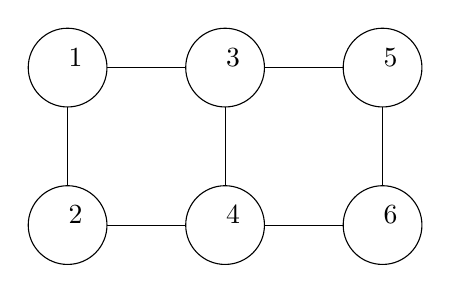
\begin{tikzpicture}
  %ノード1  
  \draw(4,2) circle (0.5)
  node[at={(4.1,2.1)}] {
    \begin{tabular}{c}
      1
    \end{tabular}
  };
  %ノード2  
  \draw(4,0) circle (0.5)
  node[at={(4.1,0.1)}] {
    \begin{tabular}{c}
      2
    \end{tabular}
  };
  %ノード3  
  \draw(6,2) circle (0.5)
  node[at={(6.1,2.1)}] {
    \begin{tabular}{c}
      3
    \end{tabular}
  };
  %ノード4  
  \draw(6,0) circle (0.5)
  node[at={(6.1,0.1)}] {
    \begin{tabular}{c}
      4
    \end{tabular}
  };
  %ノード5  
  \draw(8,2) circle (0.5)
  node[at={(8.1,2.1)}] {
    \begin{tabular}{c}
      5
    \end{tabular}
  };
  %ノード6  
  \draw(8,0) circle (0.5)
  node[at={(8.1,0.1)}] {
    \begin{tabular}{c}
      6
    \end{tabular}
  };
\draw(4,0.5) --(4,1.5);
\draw(6,0.5) --(6,1.5);
\draw(8,0.5) --(8,1.5);
\draw(4.5,0) --(5.5,0);
\draw(4.5,2) --(5.5,2);
\draw(6.5,0) --(7.5,0);
\draw(6.5,2) --(7.5,2);
\end{tikzpicture}

\caption{入力となる重み付き無向グラフの例}
\label{graphexample}
\end{center}
\end{figure}
%%%%%%%%%%%%%%%%%%%%%%%%%%%%%%

%%%%%%%%%%%%%%%%%%%%%%%%%%%%%%
\lstinputlisting[float=t,caption={%
図~\ref{graphexample}のASPファクト表現},%
captionpos=b,frame=single,label=code:graph_example.lp,%
numbers=none,%
breaklines=true,%
columns=fullflexible,keepspaces=true,%
basicstyle=\ttfamily\scriptsize]{code/graph_example.lp}
%%%%%%%%%%%%%%%%%%%%%%%%%%%%%%


本節では,最短ハミルトン閉路問題の例にとって,
入力となる重み付き無向グラフ(図~\ref{graphexample})の
ASP ファクト形式について説明する.
%
このグラフは,頂点数が6,辺の数が7であり,辺に付けられた値は距離を表す.
コード~\ref{code:graph_example.lp}に,ASPファクト形式を示す.
%
アトム\code{node/1}は頂点,\code{edge/2}は辺,\code{cost/3}は距離を表す.
例えば,\code{cost(1,2,3)}は,辺\code{edge(1,2)}の距離が3であることを
表している.

%%%%%%%%%%%%%%%%%%%%%%%%%%%%%%%%%%%%%%%%%%%%%%%%%%%%%%%%%%%%%%%%%%%%%%%
\section{ハミルトン閉路問題の ASP 符号化}\label{hamiltonianasp}
%%%%%%%%%%%%%%%%%%%%%%%%%%%%%%%%%%%%%%%%%%%%%%%%%%%%%%%%%%%%%%%%%%%%%%%

ハミルトン閉路問題は,与えられたグラフの全頂点をちょうど一度ずつ通る閉
路(ハミルトン閉路)が存在するかどうかを判定する問題である.
$G=(V,E)$にハミルトン閉路が存在する必要十分条件は,
以下の2つの制約を満たす部分グラフ$G'=(V,E')$が存在することである.

\begin{itemize}
\item $G'$の各頂点の次数が2 (次数制約)
\item $G'$が連結である (連結制約)
\end{itemize}

本論文では,前者を\textbf{次数制約},後者を\textbf{連結制約}と呼ぶ.
ハミルトン路問題は,ハミルトン閉路問題から始点と終点が一致するという閉
路の条件を取り除いたものである.
ハミルトン路問題では,次数制約は以下のように変わる.

\begin{itemize}
\item 始点と終点の次数が1,他の頂点の次数が2
\end{itemize}

以下では,ハミルトン閉路問題に対する3つの ASP 符号化
\textsf{undirected},\textsf{directed},\textsf{acyclicity}
を提案する.

%%%%%%%%%%%%%%%%%%%%%%%%%%%%%%%%%%%%%%%%%%%%%%%%%%%%%%%%%%%%%%%%%%%%%%%
\subsection{\textsf{undirected}符号化}
%%%%%%%%%%%%%%%%%%%%%%%%%%%%%%%%%%%%%%%%%%%%%%%%%%%%%%%%%%%%%%%%%%%%%%%

%%%%%%%%%%%%%%%%%%%%%%%%%%%%%%
\lstinputlisting[float=t,caption={%
\textsf{undirected}符号化},%
captionpos=b,frame=single,label=code:hamilton1.lp,%
numbers=left,%
breaklines=true,%
columns=fullflexible,keepspaces=true,%
basicstyle=\ttfamily\footnotesize]{code/hamilton1.lp}
%%%%%%%%%%%%%%%%%%%%%%%%%%%%%%

\textsf{undirected}符号化は,ハミルトン閉路問題の次数制約と連結制約を,
ASP の一貫性制約で表した基本的な符号化である.
コード~\ref{code:hamilton1.lp}に,\textsf{undirected}符号化を示す.
この符号化は,ハミルトン閉路問題とハミルトン路問題の両方に対応している.
符号化中の\code{s}は始点の頂点番号,\code{t}は終点の頂点番号を表し,こ
れらは実行時に与えられる.
ここでは,ハミルトン閉路問題(\code{s}=\code{t})の場合について説明する.

\begin{itemize}
\item 1行目のルールは,各辺\code{edge(X,Y)}に対して,その辺がハミルト
  ン閉路に含まれるかどうかを意味するアトム\code{in(X,Y)}を選択子を用い
  て導入している.
\item 次数制約は3行目のルールで表される.このルールは,
  各頂点\code{node(X)}に対して,その次数の和が2に等しいことを個数制約
  を使って表している.
\item 連結制約は11行目のルールで表される.
ある頂点\code{X}が始点\code{s}から到達可能であることを意味する補助アト
ム\code{reached(X)}を導入する.
8行目のルールは,始点\code{s}が到達可能あることを表している.
9行目のルールは,各辺\code{X}--\code{Y}に対して,その辺がハミルトン閉
路に含まれ(\code{in(X,Y)}),かつ,頂点\code{X}が始点から到
達可能であれば(\code{reached(X)}),\code{Y}も到達可能であることを表している.
10行目は9行目と同様であるが,辺\code{Y}--\code{X}の場合を表している.
11行目のルールは,各頂点\code{node(X)}が始点から到達可能でなければな
らないことを一貫性制約を使って表している.
\end{itemize}

%%%%%%%%%%%%%%%%%%%%%%%%%%%%%%%%%%%%%%%%%%%%%%%%%%%%%%%%%%%%%%%%%%%%%%%
\subsection{\textsf{directed}符号化}
%%%%%%%%%%%%%%%%%%%%%%%%%%%%%%%%%%%%%%%%%%%%%%%%%%%%%%%%%%%%%%%%%%%%%%%

%%%%%%%%%%%%%%%%%%%%%%%%%%%%%%
\lstinputlisting[float=t,caption={%
\textsf{directed}符号化},%
captionpos=b,frame=single,label=code:hamilton2.lp,%
numbers=left,%
breaklines=true,%
columns=fullflexible,keepspaces=true,%
basicstyle=\ttfamily\footnotesize]{code/hamilton2.lp}
%%%%%%%%%%%%%%%%%%%%%%%%%%%%%%

\textsf{directed}符号化は,\textsf{undirected}符号化をベースに,
与えられた無向グラフの各辺$u-v$に対して,2つの弧$u\rightarrow v$と
$v\rightarrow u$を対応させることで有向グラフ化して解く符号化である.
コード~\ref{code:hamilton2.lp}に,\textsf{directed}符号化を示す.
前節と同様に,ハミルトン閉路問題(\code{s}=\code{t})の場合について説明する.

\begin{itemize}
\item 1行目では,無向グラフの有向グラフ化を行う.
  与えられた無向グラフの各辺\code{edge(X,Y)}に対して,
  2つの弧\code{edge(X,Y)},\code{edge(Y,X)}を導入した.
\item 2行目のルールは,各弧\code{edge(X,Y)}に対して,その弧がハミルト
  ン閉路に含まれるかどうかを意味するアトム\code{in(X,Y)}を選択子を用い
  て導入している.
\item 次数制約は4,5行目のルールで表される.
  4行目では,各頂点\code{node(X)}に対して,
  その出次数が1に等しいことを個数制約を使って表している.
  5行目では,入次数について4行目と同様の制約を表す.
\item 連結制約は15行目のルールで表される.
  ある頂点\code{X}が始点\code{s}から到達可能であることを意味する
  補助アトム\code{reached(X)}を導入する.
  13行目のルールは,始点\code{s}が到達可能あることを表している.
  14行目のルールは,各弧\code{X}--\code{Y}に対して,その弧がハミルトン閉路
  に含まれ(\code{in(X,Y)}),かつ,頂点\code{X}が始点から
  到達可能であれば(\code{reached(X)}),\code{Y}も到達可能であることを表している.
  15行目のルールは,各頂点\code{node(X)}が始点から到達可能でなければ
  ならないことを一貫性制約を使って表している.
\item 18行目のルールは,解についての対称性を除去する.
  与えられた無向グラフ上の各ハミルトン閉路に対して,
  それを変換した有向グラフ上のハミルトン閉路は対称な2つが存在する.
  これによる解の重複を防ぐために,18行目のルールは,各弧\code{s}--\code{X},
  \code{Y}--\code{s}がハミルトン閉路に含まれるならば(\code{in(s,X),in(Y,s)}),
  \code{X < Y}でなければならないことを,一貫性制約を用いて表している
\end{itemize}

%%%%%%%%%%%%%%%%%%%%%%%%%%%%%%%%%%%%%%%%%%%%%%%%%%%%%%%%%%%%%%%%%%%%%%%
\subsection{\textsf{acyclicity}符号化}
%%%%%%%%%%%%%%%%%%%%%%%%%%%%%%%%%%%%%%%%%%%%%%%%%%%%%%%%%%%%%%%%%%%%%%%

%%%%%%%%%%%%%%%%%%%%%%%%%%%%%%
\lstinputlisting[float=t,caption={%
\textsf{acyclicity}符号化},%
captionpos=b,frame=single,label=code:hamilton3.lp,%
numbers=left,%
breaklines=true,%
columns=fullflexible,keepspaces=true,%
basicstyle=\ttfamily\footnotesize]{code/hamilton3.lp}
%%%%%%%%%%%%%%%%%%%%%%%%%%%%%%

\textsf{acyclicity}符号化は,\textsf{directed}符号化をベースに,
連結の制約に代わる部分閉路禁止制約を組込み非閉路制約で表現した符号化である.
コード~\ref{code:hamilton3.lp}に,\textsf{acyclicity}符号化を示す.
前節と同様に,ハミルトン閉路問題(\code{s}=\code{t})の場合について説明する.

\begin{itemize}
\item 1行目では,無向グラフの有向グラフ化を行う.
  与えられた無向グラフの各辺\code{edge(X,Y)}に対して,
  2つの弧\code{edge(X,Y)},\code{edge(Y,X)}を導入した.
\item 2行目のルールは,各弧\code{edge(X,Y)}に対して,その弧がハミルト
  ン閉路に含まれるかどうかを意味するアトム\code{in(X,Y)}を選択子を用い
  て導入している.
\item 次数制約は4,5行目のルールで表される.
  4行目では,各頂点\code{node(X)}に対して,
  その出次数が1に等しいことを個数制約を使って表している.
  5行目では,入次数について4行目と同様の制約を表す.
\item 部分閉路禁止制約は14行目のルールで表される.
  このルールは,始点でない各頂点\code{X},\code{Y}について,
  弧\code{X}--\code{Y}がハミルトン閉路に含まれるならば(\code{in(X,Y)}),
  そのような弧の集合をもつグラフが閉路をもたないことを,\code{#edge}宣言を用いて表す.
  ようするに,始点(終点)を含まないような閉路を禁止している.
\item 17行目のルールは,解についての対称性を除去する.
  与えられた無向グラフ上の各ハミルトン閉路に対して,
  それを変換した有向グラフ上のハミルトン閉路は対称な2つが存在する.
  これによる解の重複を防ぐために,17行目のルールは,各弧\code{s}--\code{X},
  \code{Y}--\code{s}がハミルトン閉路に含まれるならば(\code{in(s,X),in(Y,s)}),
  \code{X < Y}でなければならないことを,一貫性制約を用いて表している
\end{itemize}

%%%%%%%%%%%%%%%%%%%%%%%%%%%%%%%%%%%%%%%%%%%%%%%%%%%%%%%%%%%%%%%%%%%%%%% 
\section{最短ハミルトン閉路問題のASP符号化}\label{minexpl}
%%%%%%%%%%%%%%%%%%%%%%%%%%%%%%%%%%%%%%%%%%%%%%%%%%%%%%%%%%%%%%%%%%%%%%% 

%% %%%%%%%%%%%%%%%%%%%%%%%%%%%%%%
%% \lstinputlisting[caption =  最適化,label = minimize]{code/obj_minimize.lp}
%% %%%%%%%%%%%%%%%%%%%%%%%%%%%%%%

%%%%%%%%%%%%%%%%%%%%%%%%%%%%%%
\lstinputlisting[float=t,caption={%
最小化},%
captionpos=b,frame=single,label=code:obj_minimize.lp,%
numbers=left,%
breaklines=true,%
columns=fullflexible,keepspaces=true,%
basicstyle=\ttfamily\footnotesize]{code/obj_minimize.lp}
%%%%%%%%%%%%%%%%%%%%%%%%%%%%%%

最短ハミルトン閉路問題の目的関数は,
ハミルトン閉路を構成する各辺の距離の総和である.
コード\ref{code:obj_minimize.lp}は,
その目的関数の最小化を表す.
このコードは,各辺\code{edge(X,Y)}に対して,その辺がハミルトン閉路に
含まれ(\code{in(X,Y)}),その距離が\code{C}である時に(\code{cost(X,Y,C)}),
\code{C}の総和の最小化を,最小化関数を用いて表している.
.
%%%%%%%%%%%%%%%%%%%%%%%%%%%%%%
\lstinputlisting[float=t,caption={%
重み付き無向グラフの有向グラフ化},%
captionpos=b,frame=single,label=code:cost_both.lp,%
numbers=left,%
breaklines=true,%
columns=fullflexible,keepspaces=true,%
basicstyle=\ttfamily\footnotesize]{code/cost_both.lp}
%%%%%%%%%%%%%%%%%%%%%%%%%%%%%%

符号化directed,acyclicityについては,
与えられた無向グラフの各辺\code{edge(X,Y)}に対して,
2つの弧\code{edge(X,Y)},\code{edge(Y,X)}を導入した.
各辺の距離もこれに対応させるために,コード\ref{code:cost_both.lp}
を追加した.
このルールは,各辺\code{X}--\code{Y}の距離を表す\code{cost(X,Y,C)}について,
\code{cost(Y,X,C)}を導入する.
これにより,与えられた無向グラフの各辺\code{edge(X,Y)}の重み\code{C}が
2つの弧\code{edge(X,Y)},\code{edge(Y,X)}にも付与された.

%%%%%%%%%%%%%%%%%%%%%%%%%%%%%%%%%%%%%%%%%%%%%%%%%%%%%%%%%%%%%%%%%%%%%%% 
\section{コスト制約付きハミルトン閉路のASP符号化}
%%%%%%%%%%%%%%%%%%%%%%%%%%%%%%%%%%%%%%%%%%%%%%%%%%%%%%%%%%%%%%%%%%%%%%% 

%%%%%%%%%%%%%%%%%%%%%%%%%%%%%%
\lstinputlisting[float=t,caption={%
コスト制約},%
captionpos=b,frame=single,label=code:cost_constraint.lp,%
numbers=left,%
breaklines=true,%
columns=fullflexible,keepspaces=true,%
basicstyle=\ttfamily\footnotesize]{code/cost_constraint.lp}
%%%%%%%%%%%%%%%%%%%%%%%%%%%%%%

コスト制約付きハミルトン閉路問題は
ハミルトン閉路問題に,距離の総和が所与の閾値以下 (または以上) であること
を制約条件として付加した問題である.
コード\ref{code:const_constraing.lp}のルールは,その制約を表す.
ルール中の\code{c}は閾値を表し,これは実行時に与えられる.
このルールは,各辺\code{edge(X,Y)}に対して,その辺がハミルトン閉路に
含まれ(\code{in(X,Y)}),その距離が\code{C}である時に(\code{cost(X,Y,C)}),
\code{C}の総和が\code{c}以下でなければならないことを,
一貫性制約と重み付き個数制約を用いて表す.

また,\ref{minexpl}と同様に,
符号化directed,acyclicityについては,
アトム\code{cost}についても有向グラフ化に
対応させるためにコード\ref{code:cost_both.lp}を追加した.
%%%%%%%%%%%%%%%%%%%%%%%%%%%%%%%%%%%%%%%%%%%%%%%%%%%%%%%%%%%%%%%%%%%%%%%

%%% Local Variables:
%%% mode: latex
%%% TeX-master: "paper"
%%% End:

\section{実行実験}\label{chap:exp}
%%%%%%%%%%%%%%%%%%%%%%%%%%%%%%
\begin{figure*}[t]
  \centering
  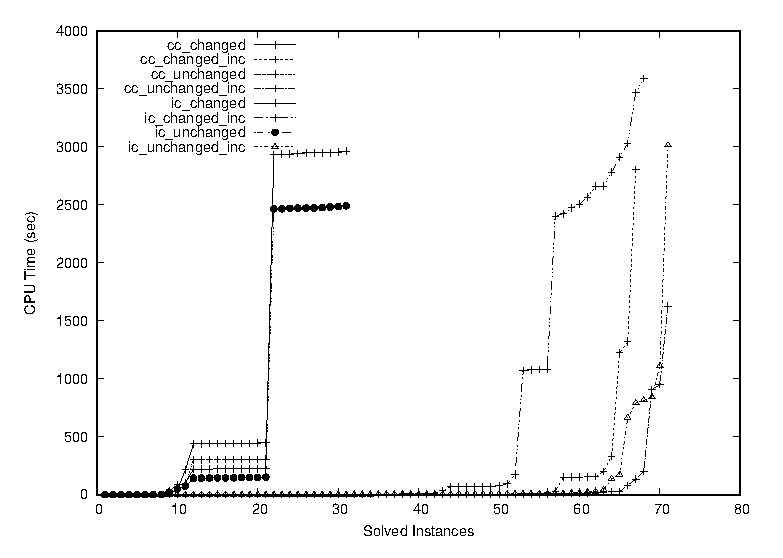
\includegraphics[scale=0.4]{fig/cactus.eps}
  \caption{基本符号化(コード~\ref{code:srf1.lp})と改良符号化(コード~\ref{code:srf2.lp})と
 発展符号化(コード~ \ref{code:srf3.lp})の比較} 
  \label{fig:cactus}
\end{figure*}
%%%%%%%%%%%%%%%%%%%%%%%%%%%%%%

%%%%%%%%%%%%%%%%%%%%%%%%%%%%%%
\begin{table*}[t]
  \caption{基本符号化(コード~\ref{code:srf1.lp})と改良符号化(コード~\ref{code:srf2.lp})と発展符号化(コード~ \ref{code:srf3.lp})の比較 (解けた問題数)} 
  \label{table:kibo}
  \centering
  \begin{tabular}[t]{rcr|c|ccc}
    \noalign{\hrule height 1pt}
    \multicolumn{3}{c|}{辺の数} & 問題数 & 基本符号化 & 改良符号化 & 発展符号化\\
    \noalign{\hrule height 1pt}
    %%%%%%%% 
       1 &~& 1000 & 30 & \textbf{30} & \textbf{30} & \textbf{30} \\ 
    1001 &~& 4000 & 20 & \textbf{20} & \textbf{20} & \textbf{20} \\ 
    4001 &~& 7000 & 11 & 9 & \textbf{10} & \textbf{10} \\ 
    7001 &~& 10000 & 8 & 4 & 6 & \textbf{8}  \\ 
    10001 &~& 20000 & 9 & 2 & 5 & \textbf{9} \\ 
    20001 &~& 30000 & 2 & 1 & \textbf{2} & \textbf{2} \\ 
    30001 &~& 40000 & 1 & 0 & 0 & \textbf{1} \\
    40001 &~& 50000 & 4 & 0 & 2 & \textbf{4} \\
    %%%%%%%% 合計
    \noalign{\hrule height 1pt}
    \multicolumn{3}{c|}{計} & 85 & 66 & 75 & \textbf{84} \\
    \noalign{\hrule height 1pt}
  \end{tabular}
\end{table*}
%%%%%%%%%%%%%%%%%%%%%%%%%%%%%%

%%%%%%%%%%%%%%%%%%%%%%%%%%%%%%
\begin{table*}[t]
  \centering
  \caption{配電網遷移問題のASP符号化(コード~\ref{code:pw-core})の実行結果}
  \label{table:core}
  \begin{tabular}{ccrrr}
 \rowcolor[RGB]{0,96,0}
\color{white}最短ステップ長 & \color{white}問題数 
     & \multicolumn{1}{c}{\color{white}シングルショット} 
         & \multicolumn{1}{c}{\color{white}マルチショット} 
             & \multicolumn{1}{c}{\color{white}シングル/マルチ} \\
 \rowcolor[RGB]{230,239,230}
1 & 6 & 1.677 & 1.035 & 1.620 \\
 \rowcolor[RGB]{196,230,196}
2 & 62 & 3.507 & 1.608 & 2.180 \\
 \rowcolor[RGB]{230,239,230}
3 & 189 & 6.089 & 2.155 & 2.826 \\
 \rowcolor[RGB]{196,230,196}
4 & 312 & 9.294 & 2.734 & 3.399 \\
 \rowcolor[RGB]{230,239,230}
5 & 280 & 13.338 & 3.361 & 3.968 \\
 \rowcolor[RGB]{196,230,196}
6 & 130 & 18.303 & 4.165 & 4.394 \\
 \rowcolor[RGB]{230,239,230}
7 & 21 & 24.483 & 5.086 & 4.814 \\
\noalign{\hrule height 0.5pt}
 \rowcolor[RGB]{196,230,196}
計 & 1000 & 76.691 & 20.114 & 3.807 \\
\end{tabular}


\end{table*}
%%%%%%%%%%%%%%%%%%%%%%%%%%%%%%

提案アプローチの有効性を評価するために,
節~\ref{chap:encode}と節~\ref{chap:core}の符号化に基づくソルバー
を開発し,実行実験を行った.

\textbf{根付き全域森問題.}
ベンチマークとしては,
DNET~\footnote{\url{https://github.com/takemaru/dnet}}
で公開されている配電網問題3問,および,
Graph Coloring and its Generalization~\footnote{\url{http://mat.tepper.cmu.edu/COLOR04/}}
で公開されているグラフ彩色問題をもとに生成した82問\footnote{%
グラフ彩色問題127問の中から,連結グラフで辺の数が50,000以下である
82問を使用した.根については全ノードの1/5をランダムに選んで使用した.
}を使用した.
ベンチマーク問題(計85問)の規模は,
ノード数11〜1406,辺の数16〜49629,根ノード数1〜281である.
%
ASPシステムには {\clingo}-5.4.0 (\textit{trendy})を使用し,
問題1問あたりの制限時間は1時間とした.
実験環境は,Mac mini,3.2 GHz Intel Core i7,64GB メモリである.

基本符号化と改良符号化と発展符号化の比較結果を
図~\ref{fig:cactus}に示す.
この図はカクタスプロットと呼ばれ,
縦軸がCPU時間,横軸が解けた問題数を表す.
グラフが下に寄るほどより高速に,右に寄るほどより多くの問題を解いたこと
を意味する.
図~\ref{fig:cactus}より,発展符号化は,他2つの符号化と比較して,より多く
の問題を高速に解いていることがわかる.

表~\ref{table:kibo}は,解けた問題数を,ベンチマーク問題に含まれる辺の数
で分類したものである.
発展符号化は,ほぼ全てのベンチマーク問題(85問中84問)が解けており,
大規模な問題に対する有効性が確認できた. 

\textbf{配電網遷移問題.}
ベンチマークとしては,DNETで公開されている実用規模の配電網問題
({\sf fukui-tepco},ノード数 432,根ノード数 72,電流上限 300)をベースにした.
この問題の実行可能解から,スタート状態を10個,ゴール状態を100個,
をランダムに選び,それらを組み合わせた計1000問の配電網遷移問題を生
成した.ASPシステムと実験環境は上と同じである.

配電網遷移問題のASP符号化(コード~\ref{code:pw-core.lp})の実行結果を
表~\ref{table:core}に示す.
左から順に,
問題名,
解を求めるまでのステップ長,解けた問題数,平均CPU時間を示している.
今回行った実行実験では,最長でステップ長が7の問題を解くことができた.


%%% Local Variables:
%%% mode: japanese-latex
%%% TeX-master: "paper"
%%% End:

%%%%%%%%%%%%%%%%%%%%%%%%%%%%%%%%%%%%%%%%%%%%%%%%%%%%%%%%%% 
\chapter{結論}
%%%%%%%%%%%%%%%%%%%%%%%%%%%%%%%%%%%%%%%%%%%%%%%%%%%%%%%%%%

XXX

%%% Local Variables:
%%% mode: latex
%%% TeX-master: "paper"
%%% End:

% ここまで

%%%%%%%%%%%%%%%%%%%%%%%%%%%%%%%%%%%%%%%%%%%%%%%%%%%%%%%%%% 
\chapter*{謝辞}
%%%%%%%%%%%%%%%%%%%%%%%%%%%%%%%%%%%%%%%%%%%%%%%%%%%%%%%%%%

%%% Local Variables:
%%% mode: japanese-latex
%%% TeX-master: "paper"
%%% End:         % 謝辞

\bibliographystyle{jplain} % 参考文献スタイル
\bibliography{bachelor,aisat}    % 参考文献リスト

\end{document}
%%%%%%%%%%%%%%%%%%%%%%%%%%%%%%%%%%%%%%%%%%%%%%%%%%%%%%%%%%

%%% Local Variables:
%%% mode: japanese-latex
%%% TeX-master: t
%%% End:
